\chapter{Data processing}
\label{ch:data_processing}

\section{Online processing}
% On the HiSPARC PC
% This data is sent to/stored in the datastore (Table 3.1 Fokkema);
% ext_timestamp
% data_reduction
% trigger_pattern
% baseline
% std_dev
% n_peaks
% pulseheigts
% integrals
% traces
% event_rate

When the \hisparc electronics trigger the detected signal traces and timing information is send to the controlling PC. First the PC determines the /gps timestamp for the event. The PC then analyses each trace individually to determine the event properties. There is a high probability (how high?) that the start of the traces (the pre-trigger window) do not contain significant signals, this is used to determine the baseline of the trace. After the baseline is known other properties can be determined.

The pulse height is the value of the highest signal in the trace, relative to the baseline. The pulse integral is the sum of the signals that are at least \SI{20}{\adc} (baselineThreshold) above the baseline. This threshold filters signal noise and small peaks.

\begin{figure}
    \centering
    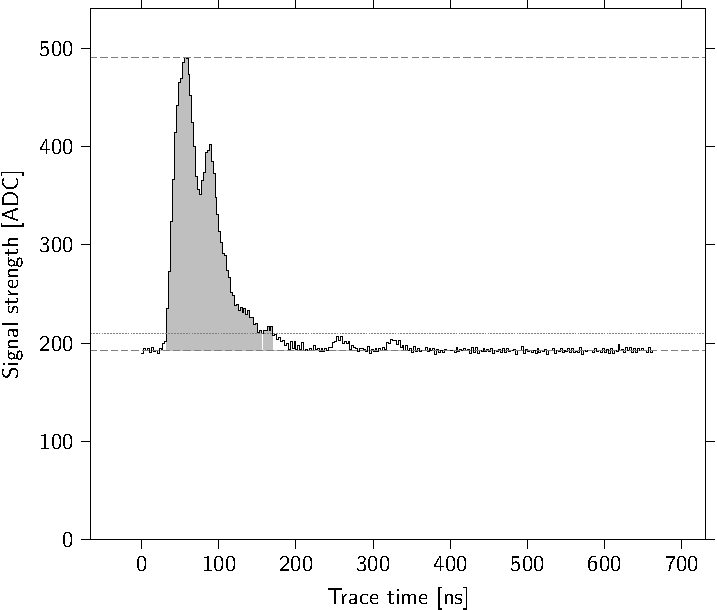
\includegraphics[width=0.7\linewidth]{plots/processing/integral}
    \caption{Illustrated definition of the pulse integral.}
    \label{fig:integral}
\end{figure}

For the number of peaks a different[?] threshold is set. As soon as the values rise above the threshold a peak is counted, when the signal reached its highest point and then drops down again the value needs to drop at least the value of the threshold before a new peak can start, for which the value needs to rise at least the threshold value again, above the new local minimum.

The standard deviation of the trace values relative to the baseline is determined.

The trigger rate (Hz) as measured by the \daq over the last 90 seconds is added to the event. The first few events when starting the \daq will have a ... to low trigger rate due to the lack of information from the 90 seconds preceding the first trigger... something like that..


\subsection{Data reduction}

\cite{oostenbrugge2014daq}

For all traces (for each channel) in an event the part which contains all significant pulses is calculated. A bit of padding is added to allow verification of the baseline in the offline analysis. The rest of the traces is cut away. On average (median) this leads to traces with \SI{150}{\ns} length. The default trace length (pre-trigger, trigger, post-trigger windows) is \SI{6}{\micro\second} (i.e. 2400 samples), so overall only \SI{2.5}{\percent} of the measured data is kept. This reduces the size of data to be transfered to the datastore and to be analysed offline. In order to have more baseline information every \SI{40}{\minute} the full traces of an event are kept. This allows for a quality check of the baselines.

% Scipt to determine some values, to be determined for larger dataset:
% lengths = [zlib.decompress(s.blobs[i]).count(',') for i in range(0, s.blobs.nrows, 4)]
% median(lengths)
% mean([l for l in lengths if l != 2400])
% len([l for l in lengths if l ==2400])


\subsection{Mean/Noise filter}

During the setup of a station the separate \adcs for each channel in the \hisparc electronics are aligned, however, this alignment is not perfect and can change over time. Typically a saw-tooth pattern can be observed in the measured traces. This can be filtered by averaging the signal. This is a multi-step process. First the trace is split in the positive and negative (adc clock) part which are smoothed seperately. These smoothed signals are interleaved again and then smoothed again. The smoothing algorithm can be configured to prevent smoothing of signals significantly different from surrounding signals, in order to preserve real pulses. Since data is compressed when stored the smoothing can improve the compressability of the data, because the data will have more equal values.

This is a destructive method in which information is lost. For the \hisparc stations at the Science Park the filtering has been disabled so raw trace values are preserved. The importance of this is described in the next section. The most recent version of the \hisparc \daq [to be released] implements this filter only for the display on the \hisparc PC. The data will be sent to the datastore unfiltered. If desired the filter can be applied in the offline analysis.

figure of raw -> filtered traces


\subsection{Trigger pattern}

The \hisparc events contain a trigger pattern which indicates which trigger thresholds were active during the trigger window, which of the comparators were triggered, and the prescense of a slave. The trigger threshold pattern does not mean that those active thresholds actually contributed to the trigger. For instance 2 simultaneous high signals in channels 1 and 2 caused a trigger, then some nano seconds later (still in the trigger window) a high signal appears in channel 3, the high threshold for channel 3 will be marked as active, even though that channel did not actively contribute to the trigger. The trigger pattern was only recently implemented (2015), along with support for the comperators.


\section{Offline processing}

Every morning, several hours after midnight, data from the previous day is processed to generate the Event Summary Data (ESD). The event processing also looks for older dates with new events, not just yesterday. Several hours after midnight is used because some stations may be slow in uploading data, this allows for some extra time to let all events from the previous day come in. Stations have a local buffer in case they are temporarily unable to upload data. There have been cases where a station had several months worth of data locally. The processing applies the event processing module from \sapphire to the data.

\subsection{Number of particles}

First data is sorted by timestamp and duplicate events are removed. Then the Most Probable Value (MPV) for the pulse integrals for each channel is determined by fitting [a gauss? check FindMPV.. class]. This provides an estimate for the signal corresponding to a single particle for that detector.

figure of pulse integral histogram


\subsection{Trigger time}

Then the trigger time for each event and the first particle in each channel is determined. We already have the \gps timestamp (upto nanoseconds) and a trace, but the timestamp is determined at the moment the trigger conditions are met.

figure showing  relative trace time (sample)  in relation to GPS time.


\subsection{Detector offsets}

Time offsets are observed between detectors, these need to be corrected for correct direction reconstruction. One day of data is enough to determine these offsets for the detectors within one station. All events that triggered a combination of two detectors. Calculate at all arrival time differences. Ideally the mean would be \SI{0}{\ns}, standard deviation related to the distance between the detectors. However, there is often an offset of several nano seconds. Distribution of offsets.. see section station.


\subsection{Coincidences}

Finally all processed events from one day are taken into one long list and coincidences are found. A coincidence is a group of least two events whos (extended) timestamps are within \SI{10000}{\ns}.


\subsection{Station offsets}

To do.
